\documentclass[dvipdfmx]{jsarticle}
\usepackage{p2report}

\begin{document}

\section{数値計算による実験方法の検討}

図\ref{fig: theoretical: reflectivity calculated}に示すようにミラーの反射率、透過率は中性子の波長$\lambda$や入射角$\theta$に大きく依存するため、手計算で実験結果を予測するのは非現実的である。
そこで実験に先立ち、
\begin{itemize}
    \item 波動関数の直接計算による確率分布の計算
    \item 確率分布に基づくモンテカルロシミュレーション
\end{itemize}
を行った。



\subsection{波動関数の直接計算}
\label{sec: simulate: theoretical}

はじめに、波動関数を直接計算して\eqref{eq: theoretical: oscillation lambda}の$\mathscr{O}(\lambda)$の分布を計算した。
計算は
\begin{enumerate}
    \item 波長を決定
    \item \eqref{eq: theoretical: R and T}からミラーの反射率・透過率を計算
    \item 図\ref{fig: theoretical: alpha and paths}点EにおけるHビーム、Oビームの波動関数を計算
    \item ビームの検出確率を計算
    \item $\mathscr{O}(\lambda)$を計算
    \item $\mathscr{O}(\lambda)$を高速フーリエ変換
\end{enumerate}
の順に行った。
図\ref{fig: simulate: reflectivity at theta 1.05}をもとに、$\mathscr{O}(\lambda)$のフーリエ変換は反射率が安定する$\SI{7e-10}{m}\leq\lambda\leq\SI{8e-10}{m}$の範囲で行う。
シミュレーション結果は測定時間無限大に相当する。

\begin{figure}
    \centering
    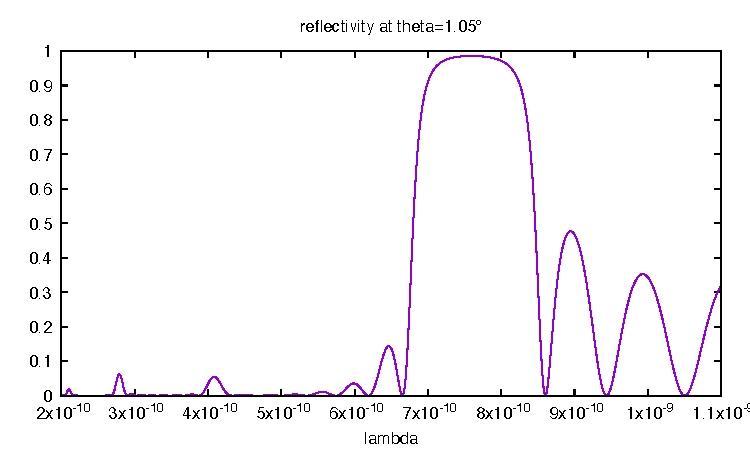
\includegraphics[width=0.6\linewidth]{img/reflNiTi-sim2.pdf}
    \caption{入射角$\theta=1.05^\circ$におけるミラーの反射率。}
    \label{fig: simulate: reflectivity at theta 1.05}
\end{figure}

$\delta, \alpha$を変えて計算したところ、$\mathscr{O}(\lambda)$のフーリエ変換は図\ref{fig: simulate: theoretical FFTs}のようになった。

\begin{figure}
    \centering
    \begin{tabular}{cc}
        \begin{minipage}{.47\linewidth}
            \centering
            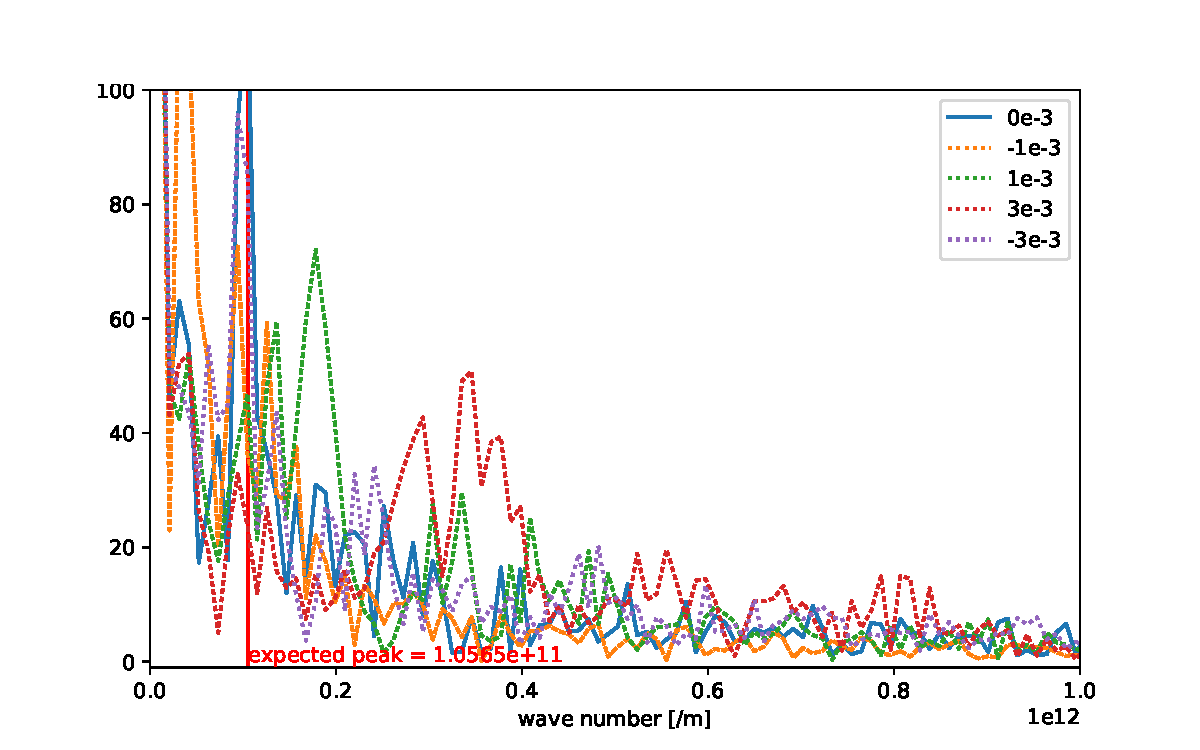
\includegraphics[width=1.\linewidth]{img/delta10.pdf}
            \subcaption{$\delta=10^\circ$}
        \end{minipage}
        &
        \begin{minipage}{.47\linewidth}
            \centering
            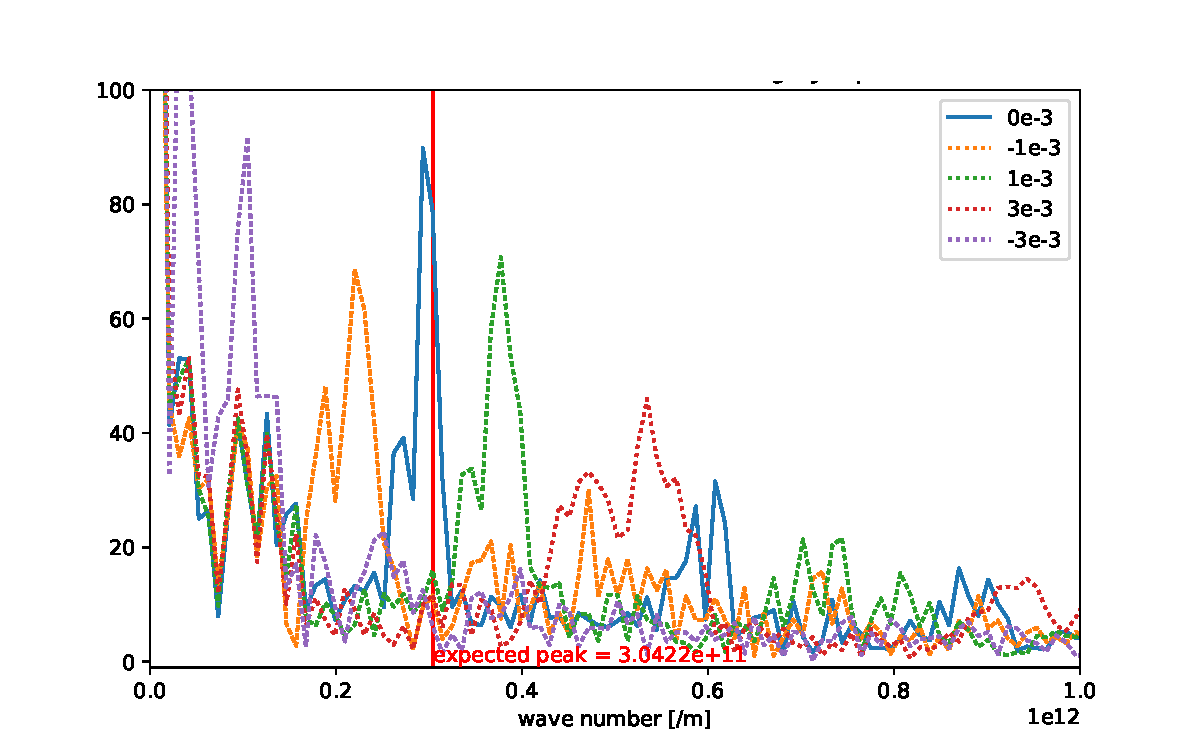
\includegraphics[width=1.0\linewidth]{img/delta30.pdf}
            \subcaption{$\delta=30^\circ$}
        \end{minipage}
        \\
        \begin{minipage}{.47\linewidth}
            \centering
            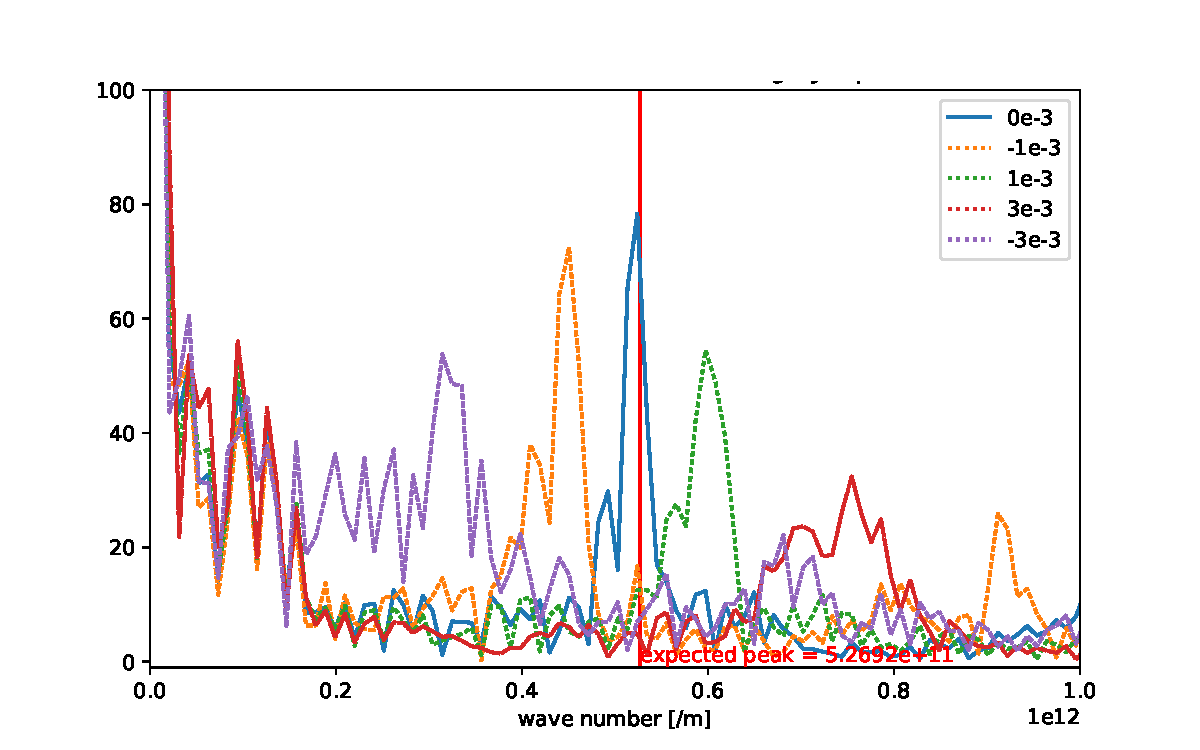
\includegraphics[width=.95\linewidth]{img/delta60.pdf}
            \subcaption{$\delta=60^\circ$}
        \end{minipage}
        &
        \begin{minipage}{.47\linewidth}
            \centering
            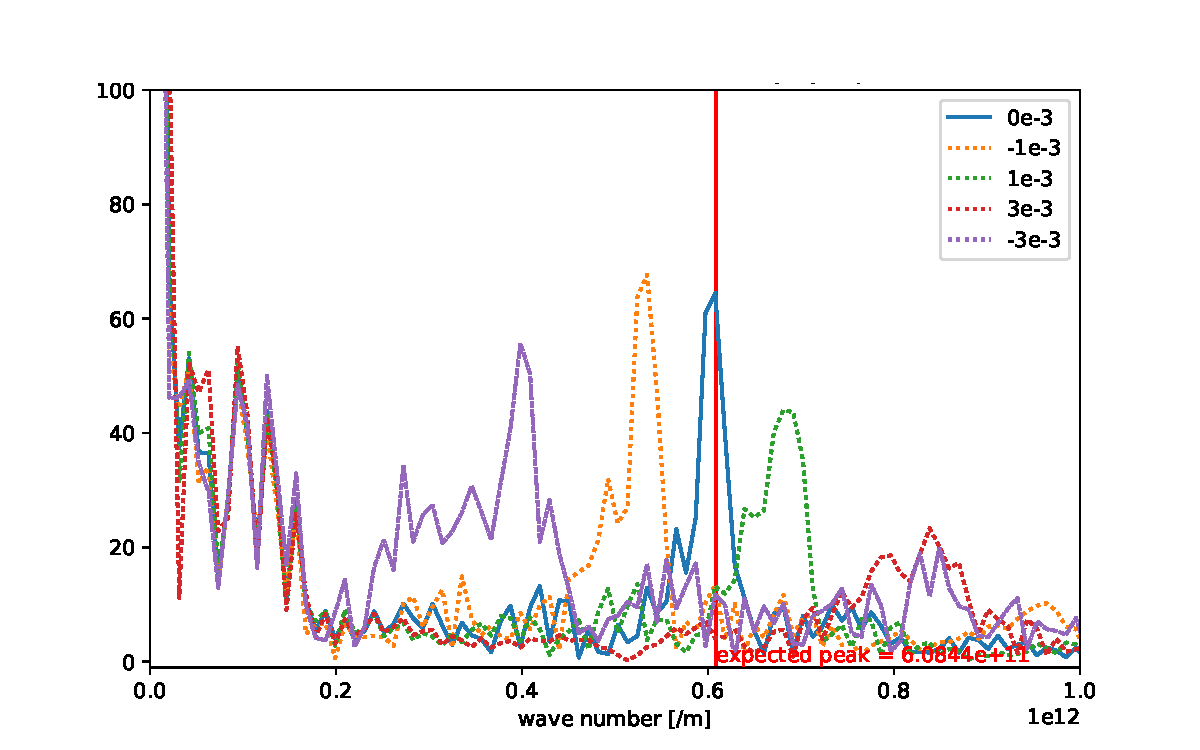
\includegraphics[width=1.\linewidth]{img/delta90.pdf}
            \subcaption{$\delta=90^\circ$}
        \end{minipage}
    \end{tabular}
    \caption{
        $\mathscr{O}(\lambda)$のフーリエ変換。
        赤の縦線は\eqref{eq: theoretical: delta phi g ideal}から予想されるピーク位置を表す。
        青の実線が$\alpha=0$の場合であり、紫、黄、緑、茶の点線がそれぞれ$\alpha=\SI{-3}{\milli\deg}, \SI{-1}{\milli\deg}, \SI{1}{\milli\deg}, \SI{3}{\milli\deg}$に対応する。
    }
    \label{fig: simulate: theoretical FFTs}
\end{figure}

$\delta$を変更しても$\SI{2e11}{\per\meter}$以下の低周波数領域がバックグラウンドとして残っている。
バックグラウンドは主にFFTを行なっている波長領域$\SI{7e-10}{\meter}\leq\lambda\leq\SI{8e-10}{\nano\meter}$におけるミラーの反射率
% や\eqref{eq: theoretical: delta phi a}の$1/\lambda$の項
から由来しているものと考えられる。
$\delta<30^\circ$ではピークがバックグラウンドと重なるため重力の効果のみを分離することが難しい。
一方で$\delta$を大きくすると特に大きい$\alpha$でピークが低く広がるため傾斜角度は小さい方が望ましい。
加えて今回用いるビームの形状とアラインメントでは$\delta>30^\circ$にてミラーの一部がビームからはみ出るため統計量を稼げなくなる。
以上を考慮して、本実験では$\delta=0$と$\delta=30^\circ$を比較することで重力の効果を検証する。


% 単結晶を用いた実験でも自重による歪みが位相に現れることが指摘されている。
% \cite{WERNER198822}\cite{COWexp}
% 本実験のセットアップでも自重によって経路が歪むことが予想されるが、以下ではこの効果を無視する。



\subsection{モンテカルロシミュレーション}
\label{sec: simulate: montecarlo}

統計誤差を見積もるため、\ref{sec: simulate: theoretical}で求めた確率分布に従いモンテカルロシミュレーションを行った。
\ref{sec: simulate: theoretical}の確率分布の計算と合わせたアルゴリズムは図\ref{fig: simulate: algorithm}の通りである。

\begin{figure}
    \centering
    \begin{tikzpicture}
        % tikz set
        \tikzset{Terminal/.style={rounded rectangle,  draw,  text centered, text width=3cm, minimum height=1.5cm}};
        \tikzset{Process/.style={rectangle,  draw,  text centered, text width=3cm, minimum height=1.5cm}};
        \tikzset{Decision/.style={diamond,  draw,  text centered, aspect=3,text width=5cm, minimum height=1.5cm}};
        % writings
        \node[Terminal](start)at(0,0){開始};
        \node[Process, below=1. of start.center](init){初期値の設定};
        \draw[->, thick]  (start) --(init);
        \node[Process, below=1.5 of init.center](lmd){各ビーム検出確率の計算};
        \draw[->, thick]  (init) --(lmd);
        \node[Decision, below=1.5 of lmd.center](particleJudge){試験粒子の検出判定};
        \draw[->, thick]  (lmd) --(particleJudge);
        \node[Process, below=.75 of particleJudge.west](particleH){H検出を記録};
        \draw[->, thick]  (particleJudge.west) --(particleH);
        \node[Process, below=.7 of particleJudge.east](particleO){O検出を記録};
        \draw[->, thick]  (particleJudge.east) --(particleO);
        \coordinate(gate1)at($(particleJudge.south)+(0,-1.25)$);
        \coordinate(gate2)at($(particleJudge.south)+(0,-1.5)$);
        \coordinate(gate3)at($(particleJudge.south)+(0,-1.75)$);
        \draw[->, thick](particleH)|-(gate1);
        \draw[->, thick](particleO)|-(gate1);
        \draw[->, thick]|-(gate2)-|($(lmd)!.4!(particleJudge)+(6,0)$)--($(lmd)!.4!(particleJudge)$)node[anchor=east]{試験粒子を波長分布に合わせてループ};
        \draw[->, thick]|-(gate3)-|($(lmd)!.5!(init)+(-6,0)$)--($(lmd)!.5!(init)$)node[anchor=west]{波長についてループ};
        \node[Terminal](end)at($(gate3)+(0,-1)$){終了};
        \draw[->, thick](particleJudge)--(end);
    \end{tikzpicture}
    \caption{
        モンテカルロシミュレーションのアルゴリズム。
        波動関数を直接計算することでビームの検出確率(3段目)を導出し、\ref{sec: simulate: theoretical}の計算に用いる。
        ビームの波長分布に合わせて試験粒子をランダムに生成し、直前で求めた各ビームの検出確率に従って検出を判定、記録する(5段目)。
        検出記録は\ref{sec: simulate: montecarlo}に使用する。
    }
    \label{fig: simulate: algorithm}
\end{figure}

ビームの波長分布に応じた個数の試験粒子を用意し、\ref{sec: simulate: theoretical}で計算した検出確率に応じてランダムに分配した。
10分に相当する粒子数で計算した結果、$\mathcal{O}(\lambda)$は図\ref{fig: simulate: oscillation of montecarlo and theoretical}のようになった。

\begin{figure}
    \centering
    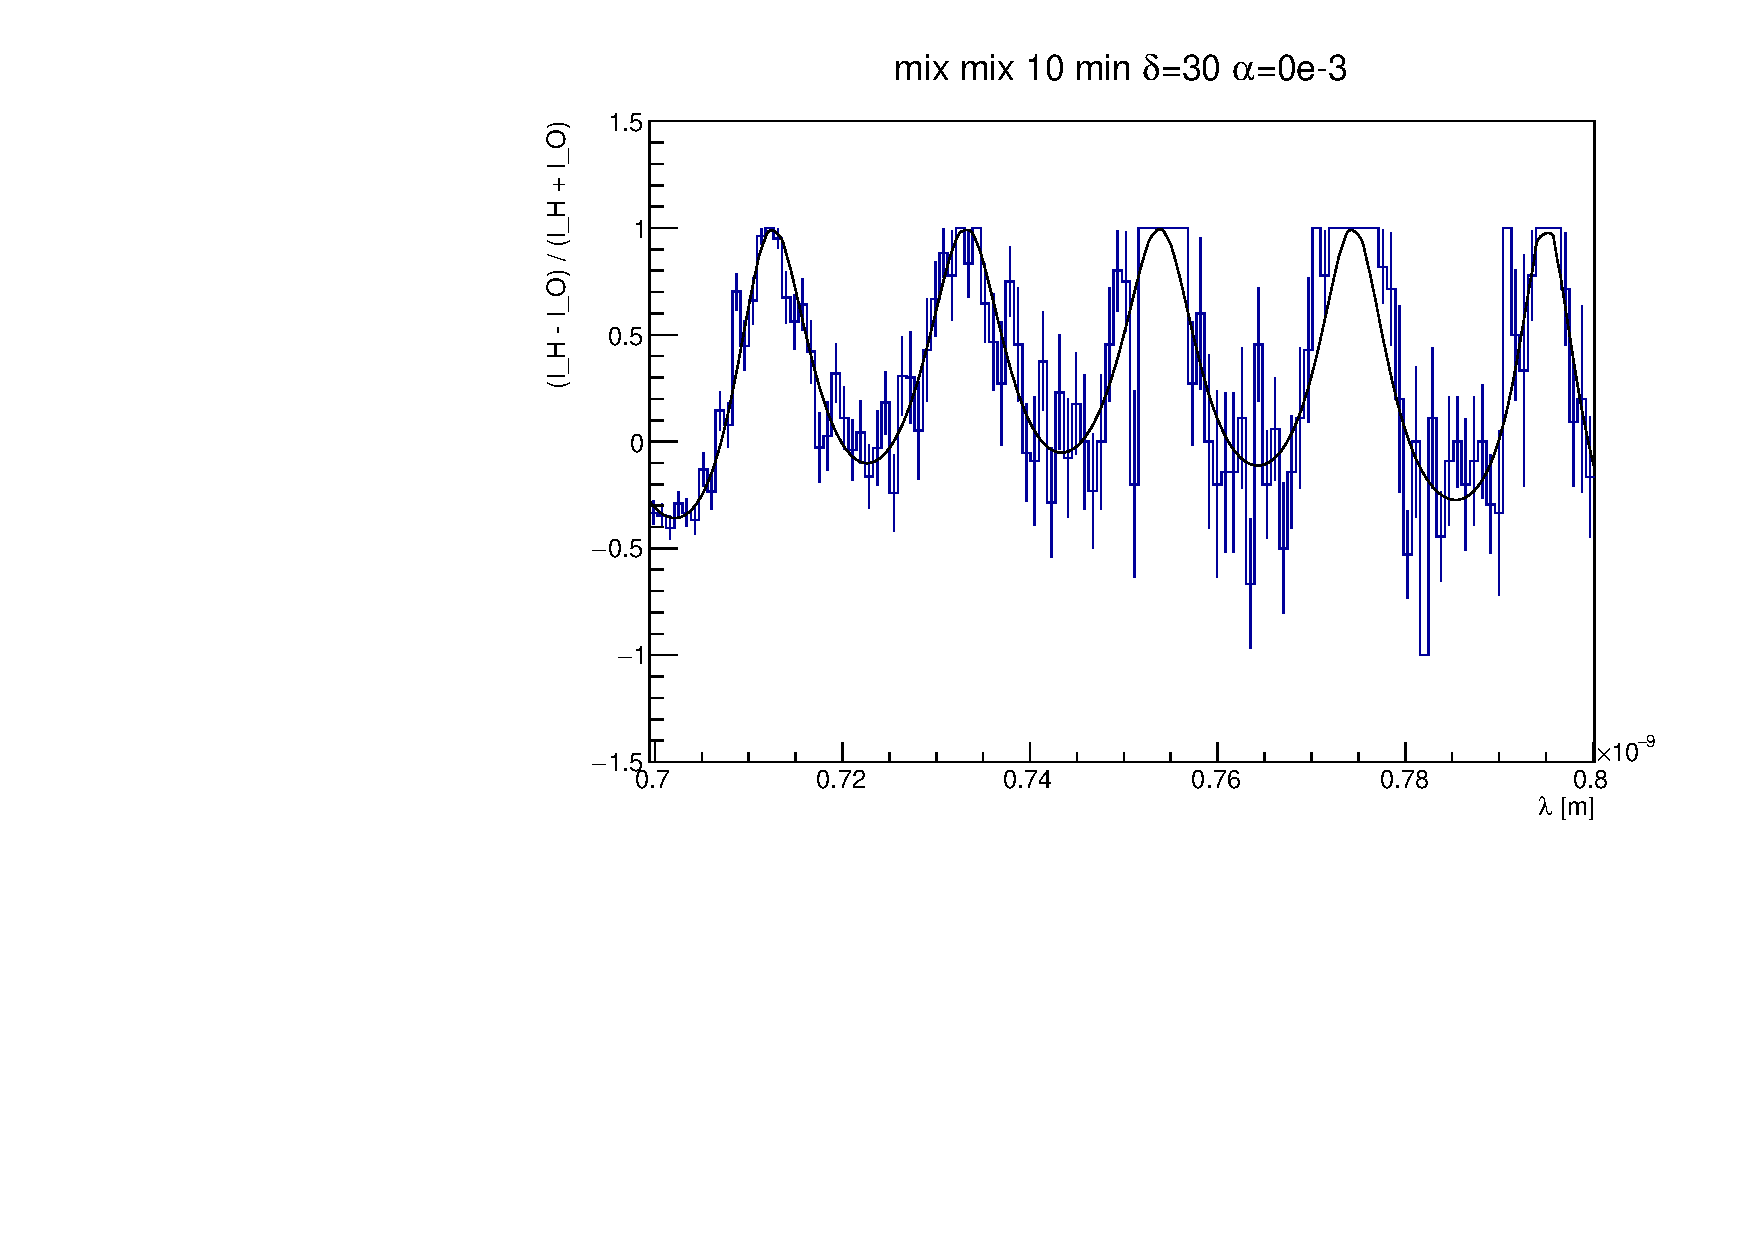
\includegraphics[width=8cm]{img/mix_mix_30deg_10min_ALPHA0e-3_lmd7e-10to8e-10.pdf}
    \caption{
        モンテカルロシミュレーションから求めた$\mathscr{O}(\lambda)$分布と理論曲線。
    }
    \label{fig: simulate: oscillation of montecarlo and theoretical}
\end{figure}

以上を踏まえて、本実験では$\delta=0$と$\delta=30^\circ$で10 min以上計測し、フーリエ成分を比較、重力加速度を逆算して$g=\SI{9.8}{m/s^2}$と照合する。

\end{document}
